% Figure for Section 6.8: Hummingbird-style clustered network.
% Build: pdflatex hb_network.tex, then copy hb_network.pdf to ../hb_network.pdf
\documentclass[border=1pt]{standalone}
\usepackage[T1]{fontenc}
\usepackage{lmodern}
\usepackage{tikz}
\usetikzlibrary{arrows.meta,decorations.pathreplacing,calc,positioning}
\definecolor{laneA}{HTML}{1F5FA8}   % lane of the source hub s
\definecolor{laneB}{HTML}{D9730D}   % lane of the relay hub s+6
\definecolor{hubgrey}{HTML}{B8B8B8}
\definecolor{inkgrey}{HTML}{4D4D4D}
\newcommand{\lb}{\sffamily\fontsize{6}{7}\selectfont}
\begin{document}
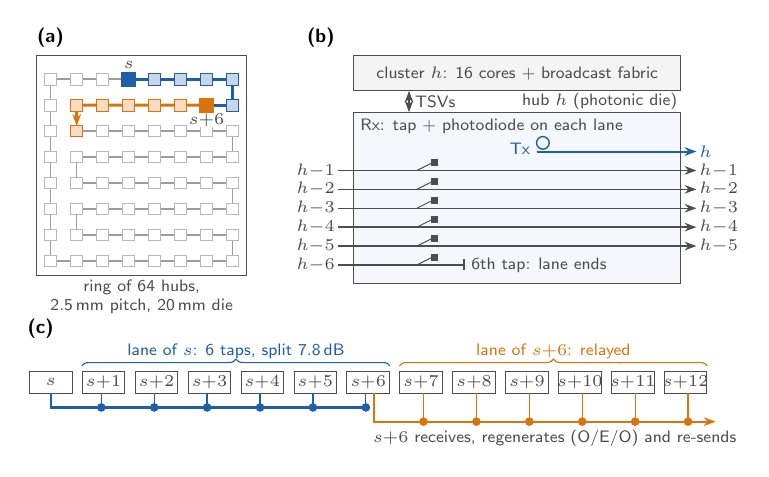
\begin{tikzpicture}[
  hub/.style={draw=inkgrey, fill=white, line width=0.35pt, minimum size=1.5mm, inner sep=0pt},
  tap/.style={circle, fill=#1, inner sep=0pt, minimum size=1.1mm},
  lbl/.style={font=\lb, text=inkgrey, inner sep=1pt},
  pl/.style={font=\sffamily\fontsize{7}{8}\selectfont\bfseries, anchor=south west, inner sep=0pt},
  >={Stealth[length=1.5mm,width=1.1mm]}]

% ================================================================== (a) the ring on the die
% A crossing-free ring through all 64 hubs of an 8x8 grid, every hop one pitch:
% along the top row, snaking through columns 1-7, and back up column 0.
\def\p{0.33}      % grid pitch in cm (2.5 mm on chip)
\foreach \i in {0,...,63}{
  \pgfmathtruncatemacro{\inrow}{\i<8}
  \pgfmathtruncatemacro{\incol}{\i>56}
  \ifnum\inrow=1
    \pgfmathtruncatemacro{\c}{\i}\pgfmathtruncatemacro{\r}{0}
  \else\ifnum\incol=1
    \pgfmathtruncatemacro{\c}{0}\pgfmathtruncatemacro{\r}{64-\i}
  \else
    \pgfmathtruncatemacro{\r}{1+int((\i-8)/7)}
    \pgfmathtruncatemacro{\q}{mod(\i-8,7)}
    \pgfmathtruncatemacro{\c}{ifthenelse(mod(\r,2)==1,7-\q,1+\q)}
  \fi\fi
  \coordinate (g\i) at ({\c*\p},{-\r*\p});
}
\draw[inkgrey!55, line width=0.5pt] (g0) \foreach \i in {1,...,63}{ -- (g\i)} -- cycle;
\foreach \i in {0,...,63}{ \node[hub, draw=hubgrey] at (g\i) {}; }
\draw[laneA, line width=1.1pt] (g3) \foreach \i in {4,...,9}{ -- (g\i)};
\draw[laneB, line width=1.1pt, ->] (g9) \foreach \i in {10,...,14}{ -- (g\i)} -- ($(g14)!0.8!(g15)$);
\foreach \i in {4,...,8}{ \node[hub, draw=laneA, fill=laneA!25] at (g\i) {}; }
\foreach \i in {10,...,15}{ \node[hub, draw=laneB, fill=laneB!25] at (g\i) {}; }
\node[hub, fill=laneA, draw=laneA, minimum size=1.8mm] at (g3) {};
\node[hub, fill=laneB, draw=laneB, minimum size=1.8mm] at (g9) {};
\node[lbl, above=0.9mm of g3] {$s$};
\node[lbl, below=0.9mm of g9, fill=white, inner sep=0.3pt] {$s{+}6$};
\draw[inkgrey, line width=0.3pt] ($(g0)+(-0.18,0.3)$) rectangle ($(g0)+({7*\p+0.18},{-7*\p-0.18})$);
\node[lbl, anchor=north, align=center] at ($(g0)+({3.5*\p},{-7*\p-0.2})$) {ring of 64 hubs,\\2.5\,mm pitch, 20\,mm die};
\node[pl] at ($(g0)+(-0.18,0.4)$) {(a)};

% ================================================================== (b) one hub, one direction
\begin{scope}[xshift=3.25cm, yshift=0.3cm]
  \node[pl] at (0,0.1) {(b)};
  % cluster above the hub
  \draw[inkgrey, fill=inkgrey!6, line width=0.3pt] (0.6,0) rectangle (4.75,-0.45);
  \node[lbl, align=center] at (2.675,-0.225) {cluster $h$: 16 cores + broadcast fabric};
  \draw[inkgrey, line width=0.4pt, <->] (1.3,-0.45) -- (1.3,-0.72) node[midway, right=1pt, lbl] {TSVs};
  \node[lbl, anchor=east] at (4.75,-0.585) {hub $h$ (photonic die)};
  % hub region on the photonic die
  \draw[inkgrey, fill=laneA!5, line width=0.3pt] (0.6,-0.72) rectangle (4.75,-2.9);
  \def\dy{0.24}
  \def\yo{-1.22}
  % receivers: one tap + photodiode per passing lane
  \node[lbl, anchor=north west] at (0.64,-0.77) {Rx: tap + photodiode on each lane};
  % own lane of h starts at its modulator
  \draw[laneA, line width=0.5pt] (3.0,\yo+0.11) circle (0.08);
  \draw[laneA, line width=0.75pt, ->] (2.92,\yo) -- (4.95,\yo);
  \node[lbl, anchor=east, text=laneA] at (2.88,\yo+0.03) {Tx};
  \node[lbl, anchor=west, text=laneA] at (4.95,\yo) {$h$};
  % lanes of h-1 ... h-5 pass through, each tapped once
  \foreach \j in {1,...,5}{
    \pgfmathsetmacro{\y}{\yo-\j*\dy}
    \draw[inkgrey, line width=0.5pt, ->] (0.4,\y) -- (4.95,\y);
    \draw[inkgrey, line width=0.35pt] (1.4,\y) -- (1.6,{\y+0.1});
    \fill[inkgrey] (1.58,{\y+0.05}) rectangle ++(0.09,0.09);
    \node[lbl, anchor=east] at (0.4,\y) {$h{-}\j$};
    \node[lbl, anchor=west] at (4.95,\y) {$h{-}\j$};
  }
  % lane of h-6: h is its sixth and last tap, so it ends here
  \pgfmathsetmacro{\y}{\yo-6*\dy}
  \draw[inkgrey, line width=0.5pt] (0.4,\y) -- (2.0,\y);
  \draw[inkgrey, line width=0.8pt] (2.0,{\y-0.07}) -- (2.0,{\y+0.07});
  \draw[inkgrey, line width=0.35pt] (1.4,\y) -- (1.6,{\y+0.1});
  \fill[inkgrey] (1.58,{\y+0.05}) rectangle ++(0.09,0.09);
  \node[lbl, anchor=east] at (0.4,\y) {$h{-}6$};
  \node[lbl, anchor=west] at (2.05,\y) {6th tap: lane ends};
\end{scope}

% ================================================================== (c) one multicast, unrolled
\begin{scope}[yshift=-3.85cm]
  \def\d{0.672}
  \node[pl] at (-0.3,0.55) {(c)};
  \foreach \j in {0,...,12}{
    \node[hub, minimum width=5.4mm, minimum height=2.8mm] (h\j) at ({\j*\d},0) {};
  }
  \node[lbl] at (h0) {$s$};
  \foreach \j in {1,...,12}{ \node[lbl, inner sep=0pt] at (h\j) {$s{+}\j$}; }
  % lane of s, tapped by s+1..s+6
  \draw[laneA, line width=0.8pt] ($(h0)+(0,-0.14)$) -- ($(h0)+(0,-0.32)$) -- ($(h6)+(-0.03,-0.32)$);
  \foreach \j in {1,...,6}{ \draw[laneA, line width=0.45pt] ($(h\j)+(-0.03,-0.32)$) -- ($(h\j)+(-0.03,-0.14)$);
                           \node[tap=laneA] at ($(h\j)+(-0.03,-0.32)$) {}; }
  % lane of s+6, tapped by s+7..s+12
  \draw[laneB, line width=0.8pt, ->] ($(h6)+(0.07,-0.14)$) -- ($(h6)+(0.07,-0.5)$) -- ($(h12)+(0.38,-0.5)$);
  \foreach \j in {7,...,12}{ \draw[laneB, line width=0.45pt] ($(h\j)+(0.03,-0.5)$) -- ($(h\j)+(0.03,-0.14)$);
                            \node[tap=laneB] at ($(h\j)+(0.03,-0.5)$) {}; }
  \draw[decorate, decoration={brace, amplitude=2.5pt}, laneA, line width=0.4pt]
       ($(h1.north west)+(0,0.06)$) -- ($(h6.north east)+(0,0.06)$)
       node[midway, above=1.5pt, lbl, text=laneA] {lane of $s$: 6 taps, split 7.8\,dB};
  \draw[decorate, decoration={brace, amplitude=2.5pt}, laneB, line width=0.4pt]
       ($(h7.north west)+(0,0.06)$) -- ($(h12.north east)+(0,0.06)$)
       node[midway, above=1.5pt, lbl, text=laneB] {lane of $s{+}6$: relayed};
  \node[lbl, anchor=north west] at ($(h6)+(0.02,-0.56)$)
       {$s{+}6$ receives, regenerates (O/E/O) and re-sends};
\end{scope}
\end{tikzpicture}
\end{document}
